\documentclass[a4paper, 11pt]{article}
\usepackage[utf8]{inputenc}
\usepackage{graphicx}
\usepackage{url}
\usepackage{hyperref}
\usepackage{color}
\usepackage{enumitem}

\title{LabSpace: A Collaborative Space where Knowledge and Experience is Shared}
\author{George E. Kallergis\\geokal@kth.se}
\date{\today{}}

\begin{document}

\maketitle

\begin{figure}[h!]
  \begin{center}
    
\includegraphics[width=\textwidth,height=\textheight,keepaspectratio]{imagery/logo.png}
    \label{fig:dneaf}
  \end{center}
\end{figure}

\textit{This document describes LabSpace, a collaborative space where students, professors, professionals and enthusiasts can exchange knowledge and experiences on a wide variety of areas including, but not limited to engineering, business, economics and art. The vision of LabSpace and its goals are discussed to allow for any interested academic organization to implement it according to its intended objectives.}

\newpage

%========%
% Introduction %
%========%
% The introduction gives an overview of the vision and goals of LabSpace.
\section*{Introduction}
LabSpace is a specially engineered maker-space \cite{whatsamakerspace} targeting the academic environment where students, professors, professionals and other enthusiasts can meet and exchange theoretical and practical knowledge around a multitude of areas of interest (engineering, business, economics, art etc.). The main vision of LabSpace is the creation of a space where knowledge is shared in a borderless fashion. A place were students can enhance their knowledge and gain experience from  professionals, teachers or even other students. The desired outcome of this is educated individuals ready to undertake challenges met in the real world, covering  the interests of the students as well as the current needs of the market. Employment rates of young professionals, innovative start up companies as well as employing companies' satisfaction levels are all expected to increase as a long term result of a LabSpace implementation.


\section{Roles} \label{sec:roles}
Figure \ref{fig:ls_env} shows LabSpace inside its preferred context. Preferred context is defined as the ideal environment into which LabSpace is expected to acomplish it's goals in an efficient and sustainable manner.

\begin{figure}[h!]
  \begin{center}
    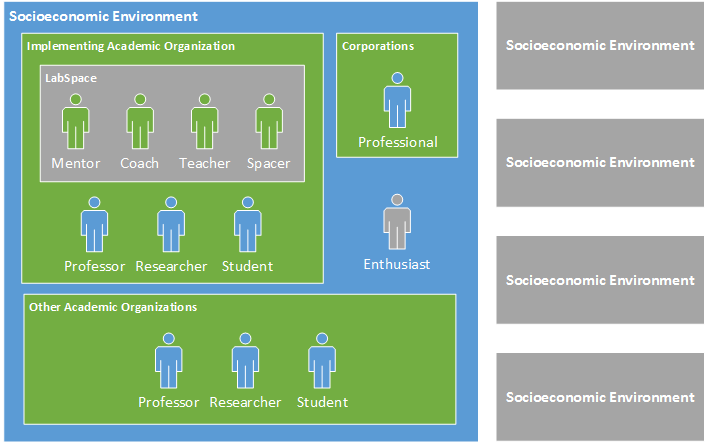
\includegraphics[width=350px,height=\textheight,keepaspectratio]{imagery/ls_context.png}
    \caption{LabSpace into the Preferred Context.}
    \label{fig:ls_env}
  \end{center}
\end{figure}

Each of the components is explained in more detail below:

\begin{itemize}[noitemsep]
    \item The \textit{implementing academic organization (IAO)} is the academic organization (i.e. the university or school) that hosts LabSpace into its premises.
    \item The \textit{socioeconomic environment} is the society and the economy into which the \textit{IAO} operates in. In other words, this block models the country the \textit{IAO} is in, along with all of its social and financial forces that affect the operation of the latter.
    \item The \textit{corporations} denote the commercial organizations that are active in that particular \textit{socioeconomic environment}.
    \item The \textit{other academic organizations} block defines other universities or schools that although they are not implementing LabSpace, they contribute to an already existing implementation sharing people and other resources. The actors in Figure \ref{fig:ls_env} define the roles different people play in the different environments inside and outside of LabSpace. 
\end{itemize}

The different roles outside of LabSpace are defined as follows:

\begin{itemize}[noitemsep]
    \item \textit{Professor}. The person that is employed as a professor in either the \textit{IAO} or any \textit{other academic organization}.
    \item \textit{Researcher}. The person that is employed as a researcher in either the \textit{IAO} or any \textit{other academic organization}.
    \item \textit{Student}. The person that is studying at either the \textit{IAO} or any \textit{other academic organization}.
    \item \textit{Professional}. The person that is or has been employed by one or more \textit{corporations} (see definition above) and is either representing his/her organization or is contributing to LabSpace as an individual.
    \item \textit{Enthusiast}. The person that belongs to none of the above categories, but still contributes to LabSpace either by providing resources or by taking part in different activities.
\end{itemize}

All of the above roles when active inside of LabSpace, turn into one (or multiple) of the following:

\begin{itemize}[noitemsep]
    \item \textit{Spacer}. The person that is learning and enhancing his/her skills inside LabSpace by participating to projects or being mentored, coached or teached by others.
    \item \textit{Mentor}. The person that is mentoring one or more spacers inside of LabSpace.
    \item \textit{Coach}. The person that is coaching one or more spacers inside of LabSpace.
    \item \textit{Teacher}. The person that is teaching one or more spacers inside of LabSpace.
\end{itemize}

Note here that multiple roles can be held by the same person inside of LabSpace. A person might be teaching someone, but at the same time being coached by someone else. Observing LabSpace from a different perspective, we could see it as a transformation of roles. Inside of LabSpace it doesn't matter if you are a professor or a student, both can teach and both should be open to learning from anybody regardless of the roles they posses outside of LabSpace. It is a neutral zone from the knowledge perspective. The additional \textit{socioeconomic environment} blocks (right hand side of Figure \ref{fig:ls_env}) define the ability of a LabSpace to cooperate on a worldwide scale regardless of the country into which the \textit{IAO} operates in.


%\begin{quote}
%    \textit{""}
%\end{quote}


%=======%
% Operation %
%=======%
% The operation section discusses the operational model of LabSpace and how an interested academic organization can go about implementing it.
\section{Operation}

The operational model defines the way the described roles interact inside (and outside) of LabSpace in order to promote its vision and accomplish its goals while sustaining the smooth operation of the space.

\subsection{The LabSpace Stakeholders}
First it is important to identify the different stakeholders of LabSpae. Stakeholders are the organizations or individuals that are immediately affected by the implementation of LabSpace and its operation. Looking at Figure \ref{fig:ls_env} we can clearly see the following stakeholders:

\begin{itemize}[noitemsep]
    \item The \textit{implementing academic organizations (IAOs)}.
    \item The \textit{students}.
    \item The \textit{professors}.
    \item The \textit{researchers}.
    \item The \textit{enthusiasts}.
    \item The \textit{professionals}.
    \item The \textit{corporations}.
    \item The \textit{socioeconomic environment}.
\end{itemize}

The \textit{IAOs} are affected by a LabSpace implementation in a number of different ways. First and foremost, they provide hosting for a particular implementation in terms of housing and other utility resources such as electricity. Secondly, the \textit{IAO} acts as a provider of key resources that are needed by an infant LabSpace implementation to begin its life. The optional IT infrastructure a LabSpace might have could also be something provided by the IAOs own infrastructure, if one exists. Finally, possible integration of LabSpace with courses provided by the \textit{IAO} and research programs undertaken by it is something that needs to be discussed with the \textit{IAO}.

The \textit{students} are the ones that have the responsibility of implementing and executing a LabSpace implementation. The viability of the space is tightly dependent on the motivation and enthusiasm shown by the students. After all, the whole idea of LabSpace is geared towards the professional and personal development of students. Most of the key activities required for the smooth operation of LabSpace are mainly carried out by the \textit{students} although cooperation with other stakeholders is always encouraged and sometimes required (e.g. when \textit{students} wish to promote a course integration with LabSpace). Taking into account the borderless knowledge exchange scheme that lives at the heart of LabSpace, \textit{students} can also act as teachers, coaches and mentors to others. Finally, they can also act as providers of key resources if they so desire.

The \textit{professors} are the ones that are expected to teach, coach and mentor the most inside of LabSpace. In the case of course and research program integrations, \textit{professors} can perform the initial steps required for the \textit{IAO} to accept and allow the execution of such a proposal. Further maintenance of such integrations is considered to be the main role of a \textit{professor} (i.e. the course material and organization inside the LabSpace context). \textit{Professors} can also act as providers of key resources if they so desire. Note here that nothing prohibits a \textit{professor} from starting and maintaining a LabSpace implementation. As long as it is in line with the LabSpace vision, anything is allowed.

The \textit{researchers}, \textit{enthusiasts} and \textit{professionals} are also expected to teach, coach and mentor inside of a LabSpace implementation bringing in theoretical and practical experience that will help towards the development of \textit{spacers}. Additionally, they can push for research program integrations with LabSpace in a way similar to the one \textit{professors} do. Finally, they could also act as providers of key resources if they so desire. Similarly, an implementation can be started by these stakeholders as well.

The \textit{corporations} are expected to bring the state of the art of their respective markets into LabSpace. Real world projects can be brought into LabSpace giving everyone the chance to work on them and gain useful practical experience. The \textit{corporations} can be active in a LabSpace implementation through \textit{professionals} they employ or through \textit{professors} (or \textit{researchers}) they cooperate with. Of course, they could also act as providers of key resources if they so desire. Due to the fact that corporations live outside of a university (unlike the rest of the stakeholders), starting a LabSpace implementation can only be done through direct cooperation with one of the aforementioned involved parties.

Finally, the \textit{socioeconomic environment} into which LabSpace is active can prove of high importance. It could act as a provider of resources (i.e. material or monetary) or as a means of raising awareness and promoting the LabSpace idea in an attempt to engage the different stakeholders mentioned above into further action. Figure \ref{fig:ls_responsibilities} summarizes all of the above.

\begin{figure}[h!]
  \begin{center}
    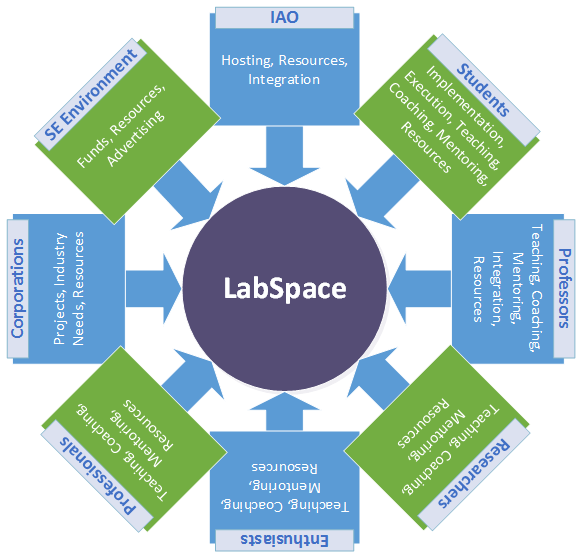
\includegraphics[width=300px,height=\textheight,keepaspectratio]{imagery/ls_stakeholders.png}
    \caption{Stakeholders' Responsibilities.}
    \label{fig:ls_responsibilities}
  \end{center}
\end{figure}

The major goal of LabSpace is the personal and professional development of students. Anything that helps in that direction is allowed and encouraged as long as the students themselves are on board with it. A proposed way of sensing the students' opinions and planning a course of action regarding a LabSpace implementation is to perform a series of studies to identify the best way to promote and achieve such an implementation in the given \textit{socioeconomic environment} and \textit{IOA}. A proposed method could be for the implementing team (regardless of whether they are students, professors or any other stakeholder capable of implementing LabSpace) to split into subteams that in parallel perform a study for each stakeholder described here. The goal of each study should be to identify the interests of each stakeholder in the specific implementation context. With that information in mind then plan for an implementation can be built. An implementation is complete when an operational model is in place that is aligned with the LabSpace vision and tries to promote the interests of all stakeholders equally within it.

Issues that should be addressed during the planning and the operational model definition phases include but are not limited to the following:

\begin{itemize}[noitemsep]
    \item Space management. Who is going to be responsible for the space itself? For example, who has the keys (if the place is in a locked area) or who is the one responsible for opening and closing the space everyday?
    \item Resources. What are the resources that we need? Which ones are already available and which ones we need to obtain? How are we going to obtain the resources that we don't have? 
    \item Resource sharing. What is the scheme of resource sharing withing the space? Can someone take artifacts home? Can someone reserve artifacts for longer periods of time, for example, to avoid rebuilding a prototype circuit on a breadboard every time they visit LabSpace?
    \item Maintenance responsibilities. Who is responsible for cleaning the space? Who is organizing the resources available so that members have easy access?
    \item Project management methods. How are the projects carried out for educational purposes going to be available to other members that didn't have the chance to work on them?
    \item Cost coverage. Is there a need for a fee to cover expenses or buying additional materials for LabSpace? Is it possible to get sponsored for some of the resources needed?
    \item Events. What kind of events are going to be carried out and in what frequency? Should there be recurring events (i.e. lectures)? Could we broadcast on-line to reach a broader audience?
    \item Cooperations. Do we need to cooperate with other LabSpaces or other student organizations to achieve our goals? How can we do that? How is going to be responsible for maintaining such relationships?
\end{itemize}

The only limit here is the creativity of the involved people in the specific LabSpace implementation. In any case, always remember that the only restriction is the LabSpace vision that demands everything to be towards the interest of the students.

\newpage

\begin{thebibliography}{9}
    \bibitem{whatsamakerspace} \emph{What’s a Makerspace?} (n.d.) [Online]. Available: \\ \href{http://makerspace.com/home-page}{http://makerspace.com/home-page} (Accessed: February 3\textsuperscript{rd}, 2014).
\end{thebibliography}

\end{document}
